% TikZ code for K^(3)(2, 2, 2) using predefined edge colors
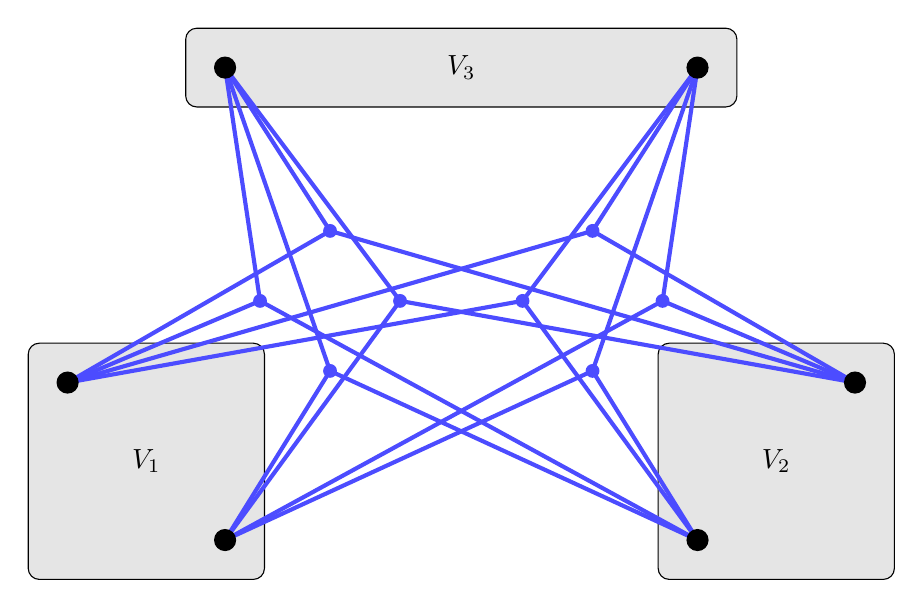
\begin{tikzpicture}[scale=1]
\draw[fill=gray!20, rounded corners] (-0.50, -0.50) rectangle (2.50, 2.50);
\node at (1.00, 1.00) [align=center] {$V_1$};
\draw[fill=gray!20, rounded corners] (7.50, -0.50) rectangle (10.50, 2.50);
\node at (9.00, 1.00) [align=center] {$V_2$};
\draw[fill=gray!20, rounded corners] (1.50, 5.50) rectangle (8.50, 6.50);
\node at (5.00, 6.00) [align=center] {$V_3$};
\coordinate (A1) at (2, 0);
\coordinate (A2) at (0, 2);
\coordinate (B1) at (8, 0);
\coordinate (B2) at (10, 2);
\coordinate (C1) at (2, 6);
\coordinate (C2) at (8, 6);
\coordinate (R0) at (3.333, 2.148);
\draw[line width=1.5pt, color=blue!70!white] (R0) -- (A1);
\draw[line width=1.5pt, color=blue!70!white] (R0) -- (B1);
\draw[line width=1.5pt, color=blue!70!white] (R0) -- (C1);
\fill[color=blue!70!white] (R0) circle (2.5pt);
\coordinate (R1) at (6.667, 2.148);
\draw[line width=1.5pt, color=blue!70!white] (R1) -- (A1);
\draw[line width=1.5pt, color=blue!70!white] (R1) -- (B1);
\draw[line width=1.5pt, color=blue!70!white] (R1) -- (C2);
\fill[color=blue!70!white] (R1) circle (2.5pt);
\coordinate (R2) at (4.222, 3.037);
\draw[line width=1.5pt, color=blue!70!white] (R2) -- (A1);
\draw[line width=1.5pt, color=blue!70!white] (R2) -- (B2);
\draw[line width=1.5pt, color=blue!70!white] (R2) -- (C1);
\fill[color=blue!70!white] (R2) circle (2.5pt);
\coordinate (R3) at (7.556, 3.037);
\draw[line width=1.5pt, color=blue!70!white] (R3) -- (A1);
\draw[line width=1.5pt, color=blue!70!white] (R3) -- (B2);
\draw[line width=1.5pt, color=blue!70!white] (R3) -- (C2);
\fill[color=blue!70!white] (R3) circle (2.5pt);
\coordinate (R4) at (2.444, 3.037);
\draw[line width=1.5pt, color=blue!70!white] (R4) -- (A2);
\draw[line width=1.5pt, color=blue!70!white] (R4) -- (B1);
\draw[line width=1.5pt, color=blue!70!white] (R4) -- (C1);
\fill[color=blue!70!white] (R4) circle (2.5pt);
\coordinate (R5) at (5.778, 3.037);
\draw[line width=1.5pt, color=blue!70!white] (R5) -- (A2);
\draw[line width=1.5pt, color=blue!70!white] (R5) -- (B1);
\draw[line width=1.5pt, color=blue!70!white] (R5) -- (C2);
\fill[color=blue!70!white] (R5) circle (2.5pt);
\coordinate (R6) at (3.333, 3.926);
\draw[line width=1.5pt, color=blue!70!white] (R6) -- (A2);
\draw[line width=1.5pt, color=blue!70!white] (R6) -- (B2);
\draw[line width=1.5pt, color=blue!70!white] (R6) -- (C1);
\fill[color=blue!70!white] (R6) circle (2.5pt);
\coordinate (R7) at (6.667, 3.926);
\draw[line width=1.5pt, color=blue!70!white] (R7) -- (A2);
\draw[line width=1.5pt, color=blue!70!white] (R7) -- (B2);
\draw[line width=1.5pt, color=blue!70!white] (R7) -- (C2);
\fill[color=blue!70!white] (R7) circle (2.5pt);
\fill[black] (A1) circle (4.0pt);
\fill[black] (A2) circle (4.0pt);
\fill[black] (B1) circle (4.0pt);
\fill[black] (B2) circle (4.0pt);
\fill[black] (C1) circle (4.0pt);
\fill[black] (C2) circle (4.0pt);
\end{tikzpicture}